\documentclass[isoft]{poster_class_UofC}

\usepackage{lipsum}
\usepackage{natbib}
\usepackage{booktabs}
\usepackage{subfig} 
\usepackage{amsmath} 
\usepackage{textcomp} 
\usepackage{url}  
\usepackage{hyperref}
\usepackage[utf8]{inputenc}
\usepackage[english]{babel}

%%%%%%%%%%%%%%%%%%%%%%%%%%%%%%%%%%%%%%%%%
%%               Configs               %%
%%%%%%%%%%%%%%%%%%%%%%%%%%%%%%%%%%%%%%%%%

% Choose one of the section color {ufglhblue | ufgdkblue | dkblue | black | gold}
\setsectioncolor{red} 
\setsubsectioncolor{gold}

% Define width of the rule or hide it by setting 0pt or commenting the command 
%\setcolumnseprule{2pt}

% Inform the paths to the logo files or leave empty one or both parameters. 
% There are three options [ T | M | B ] to positioning them.
%\setlogos[T]{images/uc-vert-rgb}

% Choose one of the background options {1 | 2 | 3}. 
% Actually, one can select any graphic file in backgrounds directory. 
\setbackground{1}

% Resize the title to keep it in two lines 
\settitlesize{64pt}{60pt}

% General info
\title{\uppercase{U-turning on Deep Learning Methods for Cell Counting:\\ A Bayesian Regression Approach}} 

\author{Andrew Pohl\textsuperscript{1}, Dylan Loader\textsuperscript{2}, Mingkuan Wu\textsuperscript{2}} 

\department{\textsuperscript{1}Faculty of Kinesiology. \textsuperscript{2}Department of Mathematics and Statistics \\ 
University of Calgary}

\email{ \text{andrew.pohl@ucalgary.ca, dylan.loader@ucalgary.ca, mingkuan@ucalgary.ca} }

%\class{Projeto Ciência no Parque}

\posteryear{2019}

\copyrightholder{Department of Mathematics and Statistics - University of Calgary}

%%%%%%%%%%%%%%%%%%%%%%%%%%%%%%%%%%%%%%%%%
%%           End configs               %%
%%%%%%%%%%%%%%%%%%%%%%%%%%%%%%%%%%%%%%%%%

\pagestyle{fancy}
\begin{document}
    \begin{poster}
    
    %%%%%%%%%%%%%%%%%%%%%%%%%%%%%%%%%%%%%%%%%
    %%             Begin poster            %%
    %%%%%%%%%%%%%%%%%%%%%%%%%%%%%%%%%%%%%%%%%
    \section{Introduction}
\begin{itemize}
\item With the invention of high throughput automated image cytometry techniques, the generation of cellular microscopy image data has accelerated drastically and automated methods are required to count cells.  

\item Current methods for cell counting are often adversely affected by deviations in image focus, by the use of differing cell staining techniques and by the fact that cells often overlap each other in images. 

\item Deep learning based image preprocessing techniques may be beneficial at improving automated methods to predict cell counts.
\end{itemize}


        
    \section{Methods}%
        
        \subsection{Dataset}
\begin{itemize}
\item The dataset consists of 3600 simulated fluorescence microscope slides obtained using 2 types of stain and 3 levels of imaging blurring, with cell counts ranging from 1 to 100 \cite{VebjornLjosa2012Ahmi}.

\item The dataset was segmented into three separate sets.  A testing set of $1200$ images was with-held by the judges.  To construct a robust training and validation environment we further segmented the training set into training (1920 images) and validation sets (480 images).
\end{itemize}
      
        \subsection{U-Net Training}
The U-Net [CITATION] is a common encoder-decoder neural network architecture which has been shown to be effective in image segmentation tasks [CITATION]. The U-Net we used to segment cells from the background of the supplied images was simplified from that used by [CITE NATURE PAPER].  It consisted of 5 layered encoder consisting of 2-dimensional convolution layers of 32,64,128,256 and 512 filters with 3x3 kernals activated by leaky rectified linear units (ReLU) Max pooling was performed between each layer, effectively halving the resolution of each feature map.  Following the encoder an equivalent 5 layer decoder network (similar but reversed layers as the encoder) was constructed with characteristic up-convolution performed immediately prior to each convolution layer.  Finally a 1 dimensional convolution layer with 1x1 kernal activated with the soft-max function was used to produce the segmentation mask for each image. The architecture for the U-Net is outlined in figure \ref{fig:U-NET}.
        
        \begin{figure}
                    \centering
            \captionsetup{type=figure}
            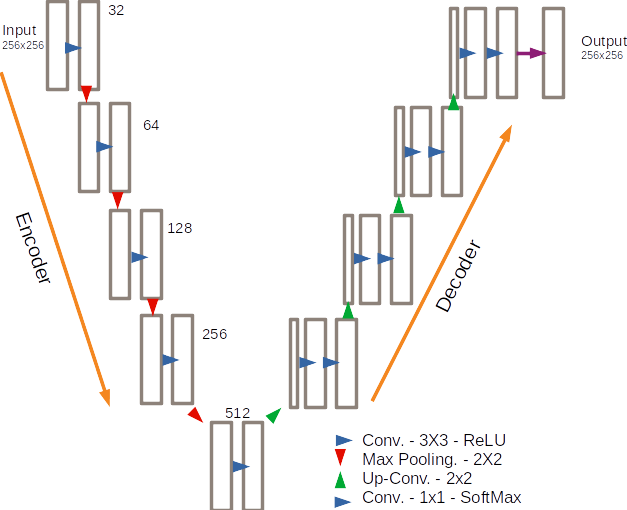
\includegraphics[scale=1]{./images/UNet_Arch.png}
            \caption{U-Net architecture used for image segmentation.}
            \label{fig:U-NET}
        \end{figure}
        
        To train the U-Net 830 images with ground-truth segmentation masks were obtained from [CITE BBBC].  NNet training was performed in Python v. 3... with the Keras interface to tensorflow \cite{chollet2015keras}.  To increase the training set size (and improve image segmentation performance) a data-generator was constructed which rescaled images to 256x256 pixels and performed random rotations along with horizontal and vertical image shifts.  The network was trained using the ADAM optimiser with a learning rate of 0.0001 and dice coefficient loss as the loss function.  Training was performed using a quad core Intel i7-7820 2.90GHz CPU.  Training was completed for 7 epochs with a batch size of 64 based on a early stopping condition when no improvement in was observed on a random 5\% validation set.  Once trained the U-Net was used to produce segmentation masks for the ... images in the respective train and validation sets used for subsequent regression analysis.  Examples of segmentation performance are shown for 3 training images in figure \ref{fig:segmentation_performance}.
        
           \begin{figure}
            \centering
            \captionsetup{type=figure}
            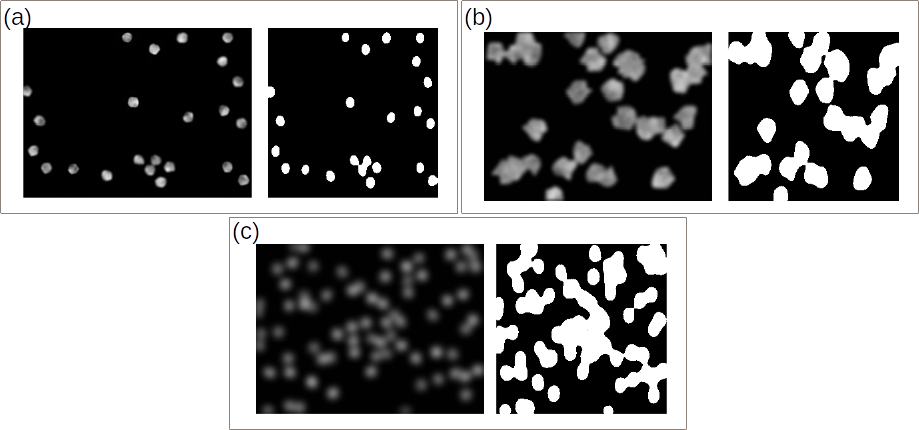
\includegraphics[scale=1.5]{./images/cell_images.png}
            \caption{Performance of Unet image segmentation for low (a), medium (b), and high (c) blur images with nulceli (a, c) and cytoplasm (b) stains.  Segmentation images are on the right with original images on the left of each block.}
            \label{fig:segmentation_performance}
        \end{figure}     
          
        \subsection{Regression Models}      
     A Bayesian implementation of polynomial regression was applied to predict the number of cells from either a raw image or U-Net generated image mask.  The sum of the normalised pixels for each image $x_i$ was used as the sole covariate to estimate cell count for each image ($y_i$).   For the U-Net generated image masks each pixel was either 0 or 1 dependent on whether the pixel was identified as a cell or not, for the raw images pixels were in the range $[0,255]$ but were subsequently normalised by dividing the observed pixel intensity by $255$ to provide pixels within the range $[0,1]$.  
     Three polynomial regression models were examined: (i) a single level model where parameter values were estimated from all images, (ii) a random slopes model where slope regression parameters ($\beta_1, \beta_2$) were allowed to vary for each stain/blur level group $j = 1, ..., 6$ and (iii) a model where both slopes ($\beta_1, \beta_2$) and intercepts ($\beta_0$) were allowed to vary for each group.  The full varying slope and intercept model is outlined in  (\ref{eqn:RegressionModel}).
\begin{align}
y_{ij} \sim N(\mu_{ij}, \sigma^2) \nonumber\\
\mu_{ij} = {\beta_0}_{j} + {\beta_1}_{j} x_{ij} + {\beta_2}_{j} x_{ij}^2 \label{eqn:RegressionModel}
\end{align}     
     Parameters of each model were estimated via Markov Chain Monte Carlo implemented in JAGS [CITE JAGS]. Weakly informative priors were utilised for each parameter. Four chains of 10000 iterations were used with convergence examined via visual examination of traceplots and determination of the R-hat and effective sample size statistics [Cite GELMAN].     
        
        \section{Results}%
The RMSE of predicting the number of cells from images within the validation is outlined in table \ref{tab:Results}.  RMSE reduces with each layer of complexity with the most complex varying slope and intercept model producing the most accurate predictions.  RMSE is similar between raw images and when image preprocessing via U-Net was implemented. image segmentation masks it is notable that performance is consistently better when raw images were used.  
        
                \vspace{1cm}
            \begin{table}
                \centering
                \captionsetup{type=table}
                \setlength{\tabcolsep}{20pt}
                \caption{Performance of regression models on validation data set}
                \label{tab:Results}
                %\renewcommand{\arraystretch}{1.2}
                \resizebox{0.5\textwidth}{!}{%
                \begin{tabular}{lccc}
				\hlinewd{3pt}
                \multirow{2}{*}{Model} & Number of & \multicolumn{2}{c}{Validation RMSE}\\
                & Parameters & Raw Images & U-Net Masks\\
                \hline
                $\mu_{ij} = {\beta_0} + {\beta_1} x_{ij} + {\beta_2} x_{ij}^2$ & 3 & 21.77 & 19.80 \\
                $\mu_{ij} = {\beta_0} + {\beta_1}_{j} x_{ij} + {\beta_2}_{j} x_{ij}^2$ & 13 & 12.45 & 13.39\\
                $\mu_{ij} = {\beta_0}_{j} + {\beta_1}_{j} x_{ij} + {\beta_2}_{j} x_{ij}^2$ & 18 & 1.74 & 1.94\\
                \hlinewd{3pt} 
                \end{tabular}
            }
            \end{table}
            \vspace{1cm}
            

There was considerable evidence to suggest differences in parameter estimates between when raw images were used vs when U-Net generated segmentation masks were used.  While this is partially explained by differing numbers of pixels between the two images sources, as outlined in figure \ref{fig:Results} U-Net segmentation had the effect of making differences between the 3 levels of blurring and two different stains become more apparent. 

             \vspace{1cm}
           \begin{figure}
            \centering
            \captionsetup{type=figure}
            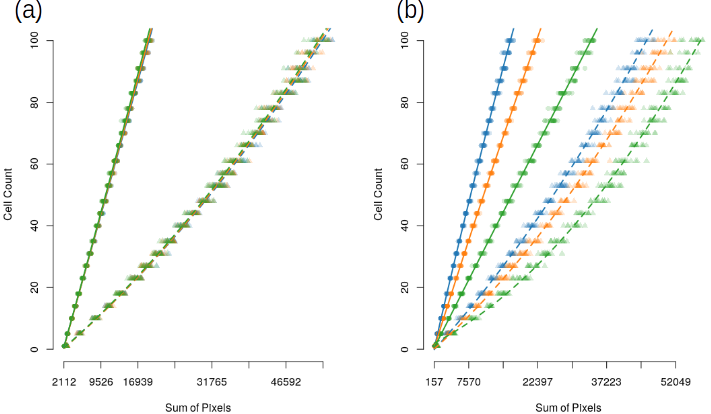
\includegraphics[scale=2]{./images/rawVUnet.png}
            \caption{Relationship between sum of pixels and cell count for (a) raw images and (b) images after U-Net segmentation processing. Low blur is indiciated in blue, medium in orange and high in green with nuclei stained images represented by circles and cell body stain represented by triangles. Fitted regression lines for the varying slopes and intercept model are included.}
            \label{fig:Results}
        \end{figure}   
            \vspace{1cm}

An advantage of using Bayesian mixed level regression models to predict cell counts is that we are able to sample from the posterior predictive distribution for the number of cells given each image in the test set.  As outlined in \ref{fig:PostPredDist} this allows us to compute a prediction interval for the likely number of cells in any given image.  Upon checking the coverage of these intervals for all images within the validation set, we can confirm such intervals are well calibrated with 95.8\% of 95\% prediction intervals containing the true cell count and intervals having an average width of 6 cells.

             \vspace{1cm}
           \begin{figure}
            \centering
            \captionsetup{type=figure}
            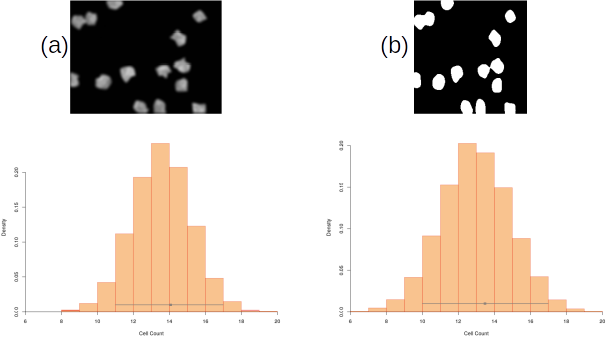
\includegraphics[scale=2]{./images/PostPredDist.png}
            \caption{Posterior predictive distribution for an image containing 14 cells when generated via the raw image (a) or U-Net segmentation mask (b).}
            \label{fig:PostPredDist}
        \end{figure}   
            \vspace{1cm}
            
    
        \section{Conclusions}
A multilevel polynomial regression model was effective in providing fairly accurate estimates of cell count along with well calibrated prediction intervals from raw microscopy images.

There was no apparent benefit to applying a segmentation mask generated by a U-Net Neural Network with regards to improving prediction performance when using polynomial regression to predict cell count.


        \section{Future Directions}
While the polynomial regression model used in this work accounts for the fact that cells are more likely to be overlapping at higher cell counts a deterministic model based off geometric properties assuming cells take fairly uniform shapes may be of benefit.  Further, modelling cell counts as normally distributed random variables is clearly an over simplification and a model based on the Gamma distribution may be more appropriate.  Finally, given their success in other image segmentation problems, alternative deep learning approaches incorporating further convolution layers and linear layers may be able to improve RMSE however these typically do not allow for adequate quantification of uncertainty as per our current Bayesian multi level regression approach. 
    
        \section{Acknowledgements}
We would like to thank Dr. Matt... for his invaluable insights in guiding this work.  We also acknowledge Mr Daniel ... for his early contribution to forming this team.

        \bibliographystyle{abbrv}
        \bibliography{refs}
    
    %%%%%%%%%%%%%%%%%%%%%%%%%%%%%%%%%%%%%%%%%
    %%               End poster            %%
    %%%%%%%%%%%%%%%%%%%%%%%%%%%%%%%%%%%%%%%%%
    
    \end{poster}

\end{document}

 
